\documentclass[aspectratio=169,11pt]{beamer}

\usepackage[T1]{fontenc}
\usepackage{lmodern}
\usepackage{booktabs}
\usepackage{listings}
\usepackage{tikz}
\usetikzlibrary{arrows.meta,positioning}
\usepackage{hyperref}

\definecolor{AmberOrange}{HTML}{D97706}
\definecolor{DeepNavy}{HTML}{123047}
\definecolor{SoftBlue}{HTML}{EAF3F8}
\definecolor{SoftAmber}{HTML}{FFF3DB}
\definecolor{Slate}{HTML}{425466}
\definecolor{Success}{HTML}{18794E}
\definecolor{Danger}{HTML}{B42318}

\setbeamercolor{normal text}{fg=DeepNavy,bg=white}
\setbeamercolor{structure}{fg=AmberOrange}
\setbeamercolor{frametitle}{fg=DeepNavy,bg=white}
\setbeamercolor{title}{fg=white}
\setbeamercolor{subtitle}{fg=SoftAmber}
\setbeamercolor{author}{fg=white}
\setbeamercolor{institute}{fg=white}
\setbeamercolor{date}{fg=SoftAmber}
\setbeamercolor{block title}{fg=white,bg=DeepNavy}
\setbeamercolor{block body}{fg=DeepNavy,bg=SoftBlue}
\setbeamercolor{alerted text}{fg=Danger}
\setbeamertemplate{navigation symbols}{}
\setbeamertemplate{footline}{%
  \leavevmode\hbox{%
  \begin{beamercolorbox}[wd=.82\paperwidth,ht=2.6ex,dp=1.2ex,leftskip=1em]{author in head/foot}%
    \color{Slate}\scriptsize AMBER2LAMMPS tutorial
  \end{beamercolorbox}%
  \begin{beamercolorbox}[wd=.18\paperwidth,ht=2.6ex,dp=1.2ex,rightskip=1em plus1fil]{date in head/foot}%
    \color{Slate}\scriptsize \insertframenumber/\inserttotalframenumber
  \end{beamercolorbox}}}
\setbeamertemplate{itemize item}{\color{AmberOrange}$\blacktriangleright$}
\setbeamertemplate{itemize subitem}{\color{AmberOrange}$\bullet$}
\setbeamersize{text margin left=8mm,text margin right=8mm}

\lstdefinestyle{terminal}{
  backgroundcolor=\color{DeepNavy},
  basicstyle=\ttfamily\footnotesize\color{white},
  breaklines=true,
  frame=single,
  rulecolor=\color{DeepNavy},
  showstringspaces=false,
  columns=fullflexible,
  keepspaces=true,
  xleftmargin=1mm,
  xrightmargin=1mm
}
\lstdefinestyle{output}{
  backgroundcolor=\color{SoftAmber},
  basicstyle=\ttfamily\scriptsize\color{DeepNavy},
  breaklines=false,
  frame=single,
  rulecolor=\color{SoftAmber},
  showstringspaces=false,
  columns=fullflexible,
  keepspaces=true,
  xleftmargin=1mm,
  xrightmargin=1mm
}
\lstdefinestyle{python}{
  language=Python,
  basicstyle=\ttfamily\footnotesize,
  backgroundcolor=\color{SoftBlue},
  breaklines=true,
  frame=single,
  rulecolor=\color{SoftBlue},
  showstringspaces=false,
  columns=fullflexible,
  keepspaces=true,
  keywordstyle=\color{AmberOrange}\bfseries,
  commentstyle=\color{Slate}
}

\title{AMBER2LAMMPS}
\subtitle{A validated workflow from AMBER topologies to LAMMPS}
\author{Arun Srikanth Sridhar}
\institute{Heriot-Watt University}
\date{Version 1.2.0}

\begin{document}

\begin{frame}[plain]
  \begin{tikzpicture}[remember picture,overlay]
    \fill[DeepNavy] (current page.south west) rectangle (current page.north east);
    \fill[AmberOrange] (current page.south west) rectangle ([xshift=0.34cm]current page.north west);
    \fill[SoftAmber,opacity=.08] ([xshift=9.8cm,yshift=-1.4cm]current page.north west) circle (3.8cm);
  \end{tikzpicture}
  \vspace{1.3cm}
  \titlepage
  \vfill
  {\color{white}\footnotesize
  \url{https://github.com/askforarun/AMBER2LAMMPS}\hfill
  DOI: 10.5281/zenodo.24348721}
\end{frame}

\begin{frame}{Learning goals}
\begin{columns}[T,onlytextwidth]
\column{0.56\textwidth}
\begin{itemize}
  \item Install the tool and fetch the example files
  \item Build a combined PDB in the right order
  \item Convert one molecule, replicas, and a GAFF2--GLYCAM mixture
  \item Choose charge targets deliberately
  \item Write a LAMMPS input that runs with the generated files
  \item Record provenance and run a bounded validation check
\end{itemize}
\column{0.40\textwidth}
\begin{block}{Starting point}
Fully parameterized AMBER \texttt{.prmtop} templates and one combined PDB with matching atom order.
\end{block}
\vspace{0.3cm}
Every command in this tutorial runs on files shipped in the repository.
\vspace{0.3cm}

\alert{The converter does not assign force-field parameters or infer cross-template covalent bonds.}
\end{columns}
\end{frame}

\begin{frame}{Conversion workflow}
\centering
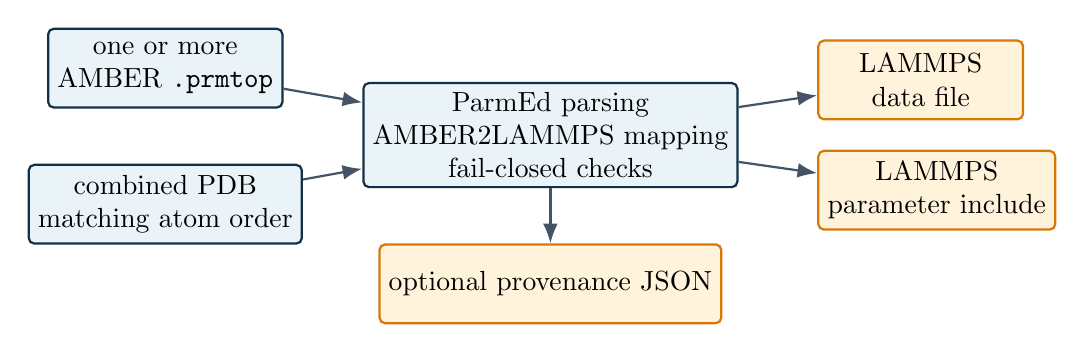
\begin{tikzpicture}[
  node distance=7mm and 10mm,
  box/.style={draw=DeepNavy,thick,rounded corners=2pt,minimum width=2.6cm,minimum height=1.0cm,align=center,fill=SoftBlue},
  outbox/.style={draw=AmberOrange,thick,rounded corners=2pt,minimum width=2.6cm,minimum height=1.0cm,align=center,fill=SoftAmber},
  arr/.style={-{Latex[length=2.5mm]},thick,draw=Slate}
]
\node[box] (top) {one or more\\AMBER \texttt{.prmtop}};
\node[box,below=of top] (pdb) {combined PDB\\matching atom order};
\node[box,right=of top,yshift=-0.85cm,minimum width=3.25cm] (convert) {ParmEd parsing\\AMBER2LAMMPS mapping\\fail-closed checks};
\node[outbox,right=of convert,yshift=0.7cm] (data) {LAMMPS\\data file};
\node[outbox,right=of convert,yshift=-0.7cm] (parm) {LAMMPS\\parameter include};
\node[outbox,below=of convert] (prov) {optional provenance JSON};
\draw[arr] (top) -- (convert);
\draw[arr] (pdb) -- (convert);
\draw[arr] (convert) -- (data);
\draw[arr] (convert) -- (parm);
\draw[arr] (convert) -- (prov);
\end{tikzpicture}
\vspace{0.6cm}

The AMBER topology remains the authoritative source of molecular-mechanics parameters.
\end{frame}

\begin{frame}[fragile]{Installation and example files}
\begin{lstlisting}[style=terminal]
python -m venv .venv
source .venv/bin/activate        # Windows: .venv\Scripts\activate
python -m pip install --upgrade pip
python -m pip install amber-to-lammps
amber-to-lammps --help

# The examples below use files from the repository
git clone https://github.com/askforarun/AMBER2LAMMPS.git
cd AMBER2LAMMPS
\end{lstlisting}

\begin{columns}[T,onlytextwidth]
\column{0.48\textwidth}
\begin{block}{Optional MCP support}
\texttt{pip install "amber-to-lammps[mcp]"}\\requires Python 3.11 or newer.
\end{block}
\column{0.48\textwidth}
LAMMPS is a separate installation. All examples need MOLECULE, KSPACE, and EXTRA-MOLECULE; 12--6--4 output also needs LEPTON.
\end{columns}
\end{frame}

\begin{frame}{Input contract}
\begin{tabular}{@{}p{0.27\textwidth}p{0.65\textwidth}@{}}
\toprule
\textbf{Input} & \textbf{Requirement} \\
\midrule
PDB & One coordinate file containing every requested molecule in template order \\
Topologies & One parameterized \texttt{prmtop} per independent molecular template \\
Counts & One molecule count per topology, in the same order \\
Charge targets & One requested net charge per topology, in the same order \\
Cell & Orthorhombic \texttt{CRYST1}, or coordinate bounds plus \texttt{--buffer} \\
\bottomrule
\end{tabular}
\vspace{0.55cm}

AMBER2LAMMPS checks list lengths, atom counts, PDB/topology atom names, cell validity, parameter completeness, and supported nonbonded combinations before writing output.
\end{frame}

\begin{frame}[fragile]{Building the combined PDB}
\begin{columns}[T,onlytextwidth]
\column{0.50\textwidth}
\begin{lstlisting}[style=terminal]
# validation/amber_family_mix/source/packmol.in
# (abridged)
tolerance 2.0
filetype pdb
output ethanol_glucose.pdb

structure ../../../ethanol.pdb
  number 1
  inside box 2.0 2.0 2.0 18.0 18.0 18.0
end structure

structure glucose.pdb
  number 1
  inside box 2.0 2.0 2.0 18.0 18.0 18.0
end structure
\end{lstlisting}
\column{0.46\textwidth}
\begin{itemize}
  \item Pack with Packmol (or build with \texttt{tleap}) from the same PDBs used to make each \texttt{prmtop}.
  \item Keep the \texttt{structure} order identical to \texttt{--topologies} and \texttt{--counts}.
  \item Add an orthorhombic \texttt{CRYST1} record for a periodic cell; otherwise the box comes from coordinates plus \texttt{--buffer}.
  \item Atom names are checked against each topology.
\end{itemize}
\alert{Avoid \texttt{--allow-pdb-name-mismatch}.}
\end{columns}
\end{frame}

\begin{frame}[fragile]{First conversion: one ethanol molecule}
\begin{lstlisting}[style=terminal]
amber-to-lammps ethanol.data ethanol.parm ethanol.pdb \
  --topologies ethanol.prmtop --counts 1 --charges 0 \
  --provenance ethanol.provenance.json
\end{lstlisting}

\begin{columns}[T,onlytextwidth]
\column{0.48\textwidth}
\textbf{Generated files}
\begin{itemize}
  \item \texttt{ethanol.data}: atoms, topology, box
  \item \texttt{ethanol.parm}: coefficients and 1--4 settings
  \item \texttt{ethanol.provenance.json}: inputs, decisions, hashes
\end{itemize}
\column{0.48\textwidth}
\textbf{Useful options}
\begin{itemize}
  \item \texttt{--verbose}: print charge and type decisions
  \item \texttt{--typelabels}: write LAMMPS type labels
  \item \texttt{--keep-temp}: write debug reports
  \item \texttt{--buffer 5.0}: box padding without \texttt{CRYST1}
\end{itemize}
\end{columns}
\end{frame}

\begin{frame}[fragile]{Replicas and mixtures use counts and templates}
\begin{lstlisting}[style=terminal]
# Ten copies of one template
amber-to-lammps ethanol10.data ethanol10.parm multi_ethanol.pdb \
  -t ethanol.prmtop -c 10 --charges 0

# Non-covalent GAFF2 ethanol + GLYCAM glucose in a 30 A cell
SRC=validation/amber_family_mix/source
amber-to-lammps mixture.data mixture.parm $SRC/ethanol_glucose.pdb \
  -t ethanol.prmtop $SRC/glucose.prmtop -c 1 1 --charges 0 0 \
  --provenance mixture.provenance.json
\end{lstlisting}

\begin{itemize}
  \item The PDB lists all copies of template 1, then all copies of template 2, and so on.
  \item Each template keeps its own active SCEE/SCNB profile.
  \item Separate templates cannot represent a covalent bond between families.
\end{itemize}
\alert{A single topology containing conflicting active 1--4 profiles is rejected.}
\end{frame}

\begin{frame}[fragile]{Why 1--4 scaling needs special treatment}
\begin{columns}[T,onlytextwidth]
\column{0.36\textwidth}
\begin{tabular}{@{}lcc@{}}
\toprule
 & \textbf{SCEE} & \textbf{SCNB} \\
\midrule
GAFF2 & 1.2 & 2.0 \\
GLYCAM06 & 1.0 & 1.0 \\
\bottomrule
\end{tabular}
\vspace{0.4cm}

LAMMPS usually applies one global \texttt{special\_bonds} rule, which cannot preserve both profiles.
\column{0.60\textwidth}
\textbf{From the generated \texttt{mixture.parm}:}
\begin{lstlisting}[style=output]
pair_style hybrid lj/cut/coul/long 9 9 &
           lj/cut/coul/long 9 9
pair_modify pair lj/cut/coul/long 1 &
  special lj 0.0 0.0 0.5 &
  special coul 0.0 0.0 0.8333333333
pair_modify pair lj/cut/coul/long 2 &
  special lj 0.0 0.0 1 special coul 0.0 0.0 1
... 66 explicit pair_coeff I J lines
\end{lstlisting}
Instance 1 carries the GAFF2 weights, instance 2 the GLYCAM weights. The mixed fixture compares every energy term and force against \texttt{sander}.
\end{columns}
\end{frame}

\begin{frame}[fragile]{A LAMMPS input that runs}
\begin{columns}[T,onlytextwidth]
\column{0.52\textwidth}
\begin{lstlisting}[style=terminal]
units real
atom_style full
boundary p p p
bond_style harmonic
angle_style harmonic
dihedral_style fourier
pair_style lj/cut/coul/long 9.0 9.0

read_data ethanol.data
include ethanol.parm

kspace_style pppm 1.0e-5
thermo_style custom step pe ebond &
  eangle edihed evdwl ecoul elong
run 0
\end{lstlisting}
\column{0.44\textwidth}
\begin{itemize}
  \item Declare the styles yourself: the parameter file sets coefficients, mixing and \texttt{special\_bonds}, but not bonded styles.
  \item For mixed or 12--6--4 output the include redefines \texttt{pair\_style}; keep the include after your own \texttt{pair\_style}.
  \item The same input runs \texttt{mixture.data}/\texttt{mixture.parm} unchanged.
\end{itemize}
\alert{Do not edit the generated \texttt{pair\_modify}, \texttt{special\_bonds}, or \texttt{pair\_coeff} lines.}
\end{columns}
\end{frame}

\begin{frame}[fragile]{Check the energies before dynamics}
\textbf{\texttt{run 0} output for the ethanol example (kcal/mol):}
\begin{lstlisting}[style=output]
   Step   PotEng      E_bond      E_angle     E_dihed       E_vdwl      E_coul      E_long
      0  -2.1616375  0.11081595  0.24613339  0.0015008588  0.15116203  27.998913  -30.670163
\end{lstlisting}
\vspace{0.3cm}
\begin{itemize}
  \item Every term should be finite and of a plausible size; inspect the components, not only \texttt{PotEng}.
  \item For a strict check, compare against \texttt{sander} on identical coordinates, as the validation fixtures do.
  \item Matching AMBER exactly also needs AMBER's Coulomb constant:
        \texttt{dielectric 1.0000346111225924} ($= 332.06371/332.0522173$).
\end{itemize}
\end{frame}

\begin{frame}[fragile]{Charge targets}
\texttt{--charges} sets the net charge of one molecule of each template.
\begin{columns}[T,onlytextwidth]
\column{0.48\textwidth}
\begin{block}{Target equals raw sum}
AMBER charges are kept unchanged. Read the raw sum with:
\end{block}
\begin{lstlisting}[style=terminal]
python -c "import parmed as p; print(sum(a.charge for a in p.load_file('ethanol.prmtop').atoms))"
\end{lstlisting}
\scriptsize ethanol: \texttt{1.0021786e-06}
\column{0.48\textwidth}
\begin{block}{Target differs from raw sum}
Every atom of that template is shifted by the same amount. \texttt{--charges 0} on ethanol shifts each atom by about $-1.1\times10^{-7}$\,e.
\end{block}
\vspace{0.2cm}
\begin{itemize}
  \item A warning is printed when the shift exceeds 0.01 e per molecule.
  \item Provenance records raw totals, targets, and shifts.
\end{itemize}
\end{columns}
\vspace{0.2cm}
\alert{AMBER2LAMMPS shifts existing charges. It never adds ions; add counterions when building the system.}
\end{frame}

\begin{frame}[fragile]{Python API}
\begin{lstlisting}[style=python]
from amber_to_lammps import amber2lammps, validate_files

src = "validation/amber_family_mix/source/"
topologies = ["ethanol.prmtop", src + "glucose.prmtop"]
counts = [1, 1]
pdb = src + "ethanol_glucose.pdb"
validate_files(topologies, counts, pdb)
amber2lammps(
    data_file="mixture.data",
    param_file="mixture.parm",
    topologies=topologies,
    molecule_counts=counts,
    pdb_file=pdb,
    charges_target=[0, 0],
    provenance_file="mixture.provenance.json",
)
\end{lstlisting}
\vspace{-0.3cm}
{\footnotesize Same engine and checks as the CLI; output identical to the CLI mixture example.}
\end{frame}

\begin{frame}{Provenance for reproducible workflows}
The JSON record captures what is needed to understand a conversion without reopening large topology or output files.

\begin{columns}[T,onlytextwidth]
\column{0.46\textwidth}
\begin{itemize}
  \item Input and output paths, sizes, SHA-256 hashes
  \item Software versions and the exact invocation
  \item Per-template counts, raw charges, and shifts
  \item Detected SCEE/SCNB profiles
\end{itemize}
\column{0.46\textwidth}
\begin{itemize}
  \item Nonbonded strategy and combination rule
  \item Box dimensions
  \item Conversion warnings
  \item Validation status (\texttt{not\_run} for a plain conversion)
\end{itemize}
\end{columns}
\vspace{0.45cm}

CLI provenance is optional. MCP conversions create it automatically. \alert{Provenance documents a conversion; it is not evidence of validation.}
\end{frame}

\begin{frame}[fragile]{Bounded MCP workflow}
\begin{lstlisting}[style=terminal]
python -m pip install "amber-to-lammps[mcp]"
amber-to-lammps-mcp
\end{lstlisting}

The local MCP server exposes two focused operations:
\begin{itemize}
  \item \textbf{convert}: run the converter inside an allowed workspace and return a compact summary
  \item \textbf{check\_lammps\_run0}: execute a bounded LAMMPS \texttt{run 0} and return energy terms or the first error
\end{itemize}

Path validation, parameter-include allowlisting, provenance hash checks, a shared execution lock, and timeouts constrain the workflow.

\alert{The MCP server does not select force fields or replace scientific review.}
\end{frame}

\begin{frame}{Validation evidence in version 1.2.0}
\small
\begin{tabular}{@{}p{0.42\textwidth}rp{0.36\textwidth}@{}}
\toprule
\textbf{Fixture} & \textbf{Atoms} & \textbf{Compared with \texttt{sander}} \\
\midrule
GLYCAM06j-1 glucose & 24 & energy terms and all forces \\
GAFF2 ethanol + GLYCAM glucose & 33 & energy terms and all forces \\
ff14SB peptide + GAFF2 ethanol & 31 & energy terms and all forces \\
ff14SB peptide + TIP3P + NaCl & 1,164 & energy terms and all forces \\
Zn(II) 12--6--4 + TIP3P + chloride & 1,020 & energy terms and all forces \\
HMR peptide + TIP3P + NaCl & 1,164 & masses, energies, forces; SHAKE setup \\
\bottomrule
\end{tabular}
\vspace{0.4cm}

CI pins AmberTools and the LAMMPS build and fails when committed tolerances are exceeded. A successful conversion alone does not count as scientific validation.
\end{frame}

\begin{frame}{Supported boundaries}
\begin{columns}[T,onlytextwidth]
\column{0.48\textwidth}
{\color{Success}\textbf{Validated examples}}
\begin{itemize}
  \item Standalone GLYCAM06j-1
  \item Non-covalent GAFF2--GLYCAM
  \item ff14SB peptide with GAFF2
  \item TIP3P water with Na$^+$/Cl$^-$
  \item Zn(II) Li/Merz 12--6--4
  \item HMR mass mapping and TIP3P SHAKE setup
\end{itemize}
\column{0.48\textwidth}
{\color{Danger}\textbf{Rejected or outside scope}}
\begin{itemize}
  \item Conflicting profiles inside one topology
  \item Mixed profiles combined with 12--6--4
  \item Cross-template covalent bonds
  \item Triclinic PDB cells
  \item Reactive or polarizable models
  \item Solute X--H constraints and HMR dynamics (not validated)
\end{itemize}
\end{columns}
\vspace{0.3cm}

Consult \texttt{docs/support-matrix.md} before extending a workflow beyond the committed fixtures.
\end{frame}

\begin{frame}{Troubleshooting checklist}
\begin{enumerate}
  \item Confirm PDB atom order matches the topology order and counts.
  \item Read warnings about charge correction and unusable \texttt{CRYST1} records.
  \item Declare bond, angle, dihedral, and pair styles before \texttt{include}; keep generated nonbonded commands intact.
  \item Check required LAMMPS packages with \texttt{lmp -h}.
  \item Run \texttt{run 0} before dynamics and inspect component energies.
  \item Preserve the provenance JSON with simulation inputs and outputs.
\end{enumerate}
\vspace{0.3cm}

For debugging, \texttt{--keep-temp} writes \texttt{<stem>.pairs.txt}, \texttt{.bonds.txt}, \texttt{.angles.txt}, and \texttt{.dihedrals.txt} beside the data file.
\end{frame}

\begin{frame}{Reproducible next steps}
\begin{itemize}
  \item Start from a validation fixture in \texttt{validation/}
  \item Reproduce its conversion and LAMMPS \texttt{run 0}
  \item Swap in your own parameterized templates and combined PDB
  \item Preserve inputs, provenance, LAMMPS script, and logs together
  \item Report unsupported physics rather than bypassing checks
\end{itemize}
\vspace{0.4cm}
\begin{block}{Resources}
\begin{tabular}{@{}ll@{}}
Repository & \url{https://github.com/askforarun/AMBER2LAMMPS} \\
PyPI & \url{https://pypi.org/project/amber-to-lammps/} \\
Archive (v1.2.0) & \url{https://doi.org/10.5281/zenodo.24348721} \\
\end{tabular}
\end{block}
\end{frame}

\begin{frame}[plain]
  \begin{tikzpicture}[remember picture,overlay]
    \fill[DeepNavy] (current page.south west) rectangle (current page.north east);
    \fill[AmberOrange] (current page.south west) rectangle ([xshift=0.34cm]current page.north west);
  \end{tikzpicture}
  \centering
  \vspace{1.5cm}
  {\color{white}\Huge Questions?}\par
  \vspace{0.7cm}
  {\color{SoftAmber}\large AMBER topology in, validated LAMMPS representation out}\par
  \vspace{1.2cm}
  {\color{white}\normalsize askforarun@gmail.com}\par
  \vspace{0.25cm}
  {\color{white}\small\url{https://github.com/askforarun/AMBER2LAMMPS}}
\end{frame}

\end{document}
